\chapter{Melarutkan Padatan Ion dan Padatan Molekul}\label{ch:g11:dissolution}

Sejumput garam yang diaduk ke dalam air lenyap dalam beberapa detik;
sejumput garam yang sama yang diaduk ke dalam minyak goreng tergeletak di
dasar gelas, tanpa berubah, selama siapa pun mau mengamatinya. Wajan
berminyak yang dibilas di bawah keran tetap berminyak; setetes sabun cuci
piring, dan minyaknya terangkat. Apa yang menentukan apakah sebuah zat
\omterm{def:g2:mixing-and-dissolving:dissolve}{larut} dalam suatu cairan? Jawabannya terletak pada \omterm{def:g11:polarity-and-cohesion:polar-bond}{muatan parsial} dan
gaya antarpartikel dari bab sebelumnya.

\begin{recall}
\omterm{def:g6:solutions-and-solubility:solubility}{Kelarutan}; cairan yang \omterm{def:g6:solutions-and-solubility:miscible}{dapat bercampur} dan yang \omterm{def:g6:solutions-and-solubility:miscible}{tidak dapat bercampur}
(\cref{ch:g6:solutions-and-solubility}). \omterm{def:g9:ions:ionic-compound}{Senyawa ion} tersusun atas
\omterm{def:g9:ions:ion}{kation} dan \omterm{def:g9:ions:ion}{anion} dalam perbandingan yang membuatnya netral
(\cref{ch:g9:ions}). \omterm{def:g11:polarity-and-cohesion:polar-molecule}{Molekul polar} dan nonpolar, \omterm{def:g11:polarity-and-cohesion:hydrogen-bond}{ikatan hidrogen},
\omterm{def:g11:polarity-and-cohesion:van-der-waals}{interaksi van der Waals} (\cref{ch:g11:polarity-and-cohesion}).
\omterm{def:g10:chemical-species:extraction}{Ekstraksi cair--cair} (\cref{ch:g10:chemical-species}). \omterm{def:g10:concentration-and-dilution:molar-concentration}{Konsentrasi molar}
(\cref{ch:g10:concentration-and-dilution}).
\end{recall}

\section{Melarutkan padatan ion}

Dalam sebutir kristal natrium klorida, setiap \omterm{def:g9:ions:ion}{ion} natrium \ce{Na+}
dikelilingi oleh \omterm{def:g9:ions:ion}{ion-ion} klorida \ce{Cl-} dan setiap \omterm{def:g9:ions:ion}{ion} klorida oleh
\omterm{def:g9:ions:ion}{ion-ion} natrium, semuanya diikat oleh tarikan antara muatan-muatan yang
berlawanan. \omterm{def:g7:atoms-and-molecules:molecule}{Molekul-molekul} air, yang polar, ditarik oleh muatan-muatan
ini: sisi oksigennya ($\delta^-$) menghadap ke \omterm{def:g9:ions:ion}{kation}, sisi hidrogennya
($\delta^+$) ke \omterm{def:g9:ions:ion}{anion}.

\begin{definition}[Disosiasi]\label{def:g11:dissolution:dissociation}
Yang disebut \emph{disosiasi}\index{disosiasi} sebuah padatan \omterm{def:g9:ions:ion}{ion} dalam
suatu \omterm{def:g6:solutions-and-solubility:solute}{pelarut} adalah terpisahnya \omterm{def:g9:ions:ion}{ion-ion} padatan itu satu dari yang
lain: \omterm{def:g9:ions:ion}{ion-ion} itu meninggalkan kristal dan saling menjauh di dalam
larutan.
\end{definition}

\begin{definition}[Solvasi, hidrasi]\label{def:g11:dissolution:solvation}
Yang disebut \emph{solvasi}\index{solvasi} sebuah partikel terlarut
adalah dikelilinginya partikel itu oleh \omterm{def:g7:atoms-and-molecules:molecule}{molekul-molekul} \omterm{def:g6:solutions-and-solubility:solute}{pelarut}, yang
terikat padanya oleh tarikan; di dalam air, solvasi disebut
\emph{hidrasi}\index{hidrasi}. Lambang (aq) sesudah sebuah rumus berarti
``terhidrasi''.
\end{definition}

\begin{proposition}[Tiga tahap pelarutan]\label{prop:g11:dissolution:stages}
Padatan \omterm{def:g9:ions:ion}{ion} \omterm{def:g2:mixing-and-dissolving:dissolve}{larut} dalam air melalui tiga tahap yang berlangsung
bersamaan: \omterm{def:g9:ions:ion}{ion-ion} ditarik keluar dari kristal (\omterm{def:g11:dissolution:dissociation}{disosiasi}), dikelilingi
\omterm{def:g7:atoms-and-molecules:molecule}{molekul-molekul} air (\omterm{def:g11:dissolution:solvation}{hidrasi}), dan tersebar ke seluruh larutan
(dispersi). Untuk natrium klorida,
\[
  \ce{NaCl(s) -> Na+(aq) + Cl-(aq)} .
\]
\end{proposition}

\begin{proof}
Diterima tanpa bukti: tarikan antara \omterm{def:g9:ions:ion}{ion-ion} dan \omterm{def:g7:atoms-and-molecules:molecule}{molekul-molekul} air
yang polar, jika dijumlahkan, cukup kuat untuk menggantikan tarikan
antara \omterm{def:g9:ions:ion}{ion-ion} di dalam kristal.
\end{proof}

\begin{omfigure}
\begin{tikzpicture}[font=\small]
  % the crystal edge: alternating ions
  \foreach \i in {0,1,2,3,4} \foreach \j in {0,1,2,3} {
    \pgfmathtruncatemacro\k{mod(\i+\j,2)}
    \ifnum\k=0
      \node[om atom, ball color=green!60!black, minimum size=6.4mm] at (0.8*\i,0.8*\j) {};
    \else
      \node[om atom, ball color=violet!70, minimum size=4.0mm] at (0.8*\i,0.8*\j) {};
    \fi
  }
  % a hydrated Na+ that has left: O towards the ion
  \begin{scope}[shift={(5.6,1.8)}]
    \node[om atom, ball color=violet!70, minimum size=4.0mm] (na) at (0,0) {};
    \node[font=\footnotesize] at (0,0) {};
    \foreach \a in {0,90,180,270} {
      \node[aO, minimum size=4.6mm] (o\a) at (\a:0.62) {};
      \node[aH, minimum size=3.2mm] (ha\a) at ($(\a:0.62)+(\a+52:0.42)$) {};
      \node[aH, minimum size=3.2mm] (hb\a) at ($(\a:0.62)+(\a-52:0.42)$) {};
      \begin{scope}[on background layer]
        \draw[bond, line width=1.2pt] (o\a.center) -- (ha\a.center);
        \draw[bond, line width=1.2pt] (o\a.center) -- (hb\a.center);
      \end{scope}
    }
    \node[anchor=north] at (0,-1.35) {\ce{Na+(aq)}};
  \end{scope}
  % a hydrated Cl- that has left: H towards the ion
  \begin{scope}[shift={(8.6,1.4)}]
    \node[om atom, ball color=green!60!black, minimum size=6.4mm] at (0,0) {};
    \foreach \a in {45,135,225,315} {
      \node[aH, minimum size=3.2mm] (h\a) at (\a:0.62) {};
      \node[aO, minimum size=4.6mm] (o\a) at (\a:1.0) {};
      \node[aH, minimum size=3.2mm] (k\a) at ($(\a:1.0)+(\a+75:0.42)$) {};
      \begin{scope}[on background layer]
        \draw[bond, line width=1.2pt] (o\a.center) -- (h\a.center);
        \draw[bond, line width=1.2pt] (o\a.center) -- (k\a.center);
      \end{scope}
    }
    \node[anchor=north] at (0,-1.45) {\ce{Cl-(aq)}};
  \end{scope}
  \node[anchor=north, align=center] at (1.6,-0.45) {kristalnya\\
    (\ce{Na+} kecil, \ce{Cl-} besar)};
\end{tikzpicture}

{\small Natrium klorida yang sedang \omterm{def:g2:mixing-and-dissolving:dissolve}{larut}. Sebuah \omterm{def:g9:ions:ion}{ion} natrium dan sebuah
\omterm{def:g9:ions:ion}{ion} klorida telah meninggalkan kristal; masing-masing terhidrasi. Di
sekeliling \omterm{def:g9:ions:ion}{kation}, \omterm{def:g7:atoms-and-molecules:molecule}{molekul-molekul} air menghadapkan \omterm{def:g7:atoms-and-molecules:atom}{atom} oksigennya
(merah, $\delta^-$) ke dalam, di sekeliling \omterm{def:g9:ions:ion}{anion} \omterm{def:g7:atoms-and-molecules:atom}{atom-atom} hidrogennya
(putih, $\delta^+$).}
\end{omfigure}

\section{Konsentrasi ion-ion}

\begin{method}[Konsentrasi setiap ion]\label{met:g11:dissolution:ions}
\begin{enumerate}
  \item Tuliskan persamaan pelarutannya, setara dalam \omterm{def:g7:atoms-and-molecules:atom}{atom} dan muatan:
        untuk kalsium klorida, \ce{CaCl2(s) -> Ca^{2+}(aq) + 2Cl-(aq)}.
  \item Hitung jumlah $n$ padatan yang dilarutkan, dan konsentrasi
        $c = n / V$ larutan terhadap \omterm{def:g6:solutions-and-solubility:solute}{zat terlarutnya}.
  \item Setiap \omterm{def:g9:ions:ion}{ion} memiliki konsentrasi $c$ dikalikan koefisiennya dalam
        persamaan: di sini $[\ce{Ca^{2+}}] = c$ dan
        $[\ce{Cl-}] = 2c$.
\end{enumerate}
Kurung siku $[\ldots]$ menyatakan \omterm{def:g10:concentration-and-dilution:molar-concentration}{konsentrasi molar} sebuah spesies yang
terlarut.
\end{method}

\begin{example}[Kalsium klorida]\label{ex:g11:dissolution:cacl2}
% ledger: aw:Ca, aw:Cl
Sebanyak \qty{5.55}{g} kalsium klorida ($M = \qty{111.1}{g/mol}$)
dilarutkan menjadi \qty{500.0}{mL} larutan: $n = \qty{0.0500}{mol}$,
$c = \qty{0.100}{mol/L}$, jadi $[\ce{Ca^{2+}}] = \qty{0.100}{mol/L}$ dan
$[\ce{Cl-}] = \qty{0.200}{mol/L}$. Larutan itu netral: $2 \times
0.100$ muatan positif per liter untuk $1 \times 0.200$ muatan negatif.
\end{example}

\section{Kepolaran dan kelarutan}

\begin{proposition}[Yang sejenis melarutkan yang sejenis]\label{prop:g11:dissolution:like}
\omterm{def:g6:solutions-and-solubility:solute}{Pelarut} polar, seperti air, melarutkan padatan \omterm{def:g9:ions:ion}{ion} dan spesies polar,
terutama yang dapat membentuk \omterm{def:g11:polarity-and-cohesion:hydrogen-bond}{ikatan hidrogen} dengannya; \omterm{def:g6:solutions-and-solubility:solute}{pelarut}
nonpolar, seperti sikloheksana atau minyak nabati, melarutkan spesies
nonpolar. Padatan \omterm{def:g9:ions:ion}{ion} sangat sedikit \omterm{def:g2:mixing-and-dissolving:dissolve}{larut} dalam \omterm{def:g6:solutions-and-solubility:solute}{pelarut} nonpolar, dan
spesies nonpolar sangat sedikit \omterm{def:g2:mixing-and-dissolving:dissolve}{larut} dalam air.
\end{proposition}

\begin{proof}
Diterima tanpa bukti: \omterm{def:g6:solutions-and-solubility:solute}{zat terlarut} \omterm{def:g2:mixing-and-dissolving:dissolve}{larut} dengan baik jika tarikan yang
dapat dibentuknya dengan \omterm{def:g6:solutions-and-solubility:solute}{pelarut} setidaknya sama kuatnya dengan tarikan
yang diputusnya, antara partikel-partikelnya sendiri dan antara
\omterm{def:g7:atoms-and-molecules:molecule}{molekul-molekul} \omterm{def:g6:solutions-and-solubility:solute}{pelarut}.
\end{proof}

\begin{example}[Tiga kasus]\label{ex:g11:dissolution:cases}
% ledger: sol:I2-water, sol:I2-heptane
Etanol bercampur dengan air dalam segala perbandingan: gugus \ce{O-H}-nya
membentuk \omterm{def:g11:polarity-and-cohesion:hydrogen-bond}{ikatan hidrogen} dengan air. Garam \omterm{def:g2:mixing-and-dissolving:dissolve}{larut} dalam air tetapi tidak
dalam minyak. Iodin, \ce{I2}, \omterm{def:g11:polarity-and-cohesion:polar-molecule}{molekul nonpolar}, sukar \omterm{def:g2:mixing-and-dissolving:dissolve}{larut} dalam air
(sekitar \qty{0.3}{g/L}, larutan cokelat) tetapi mudah \omterm{def:g2:mixing-and-dissolving:dissolve}{larut} dalam
\omterm{def:g6:solutions-and-solubility:solute}{pelarut} nonpolar (\qty{17}{g} per kilogram heptana, larutan ungu).
\end{example}

\section{Ekstraksi cair--cair, dijelaskan}

\omterm{def:g10:chemical-species:extraction}{Ekstraksi cair--cair} memindahkan sebuah spesies dari satu \omterm{def:g6:solutions-and-solubility:solute}{pelarut} ke
\omterm{def:g6:solutions-and-solubility:solute}{pelarut} lain, yang \omterm{def:g6:solutions-and-solubility:miscible}{tidak dapat bercampur} dengan \omterm{def:g6:solutions-and-solubility:solute}{pelarut} pertama, tempat
spesies itu lebih mudah \omterm{def:g2:mixing-and-dissolving:dissolve}{larut}. Aturan ``yang sejenis melarutkan yang
sejenis'' menunjukkan \omterm{def:g6:solutions-and-solubility:solute}{pelarut} mana yang harus dipilih.

\begin{inthelab}[Mengekstraksi iodin]
Sebanyak \qty{20}{mL} larutan iodin berair yang berwarna cokelat
dituang ke dalam corong pisah bersama \qty{10}{mL} sikloheksana. Corong
itu disumbat, dikocok, tekanannya dilepaskan melalui keran, lalu
didiamkan. Terbentuk dua lapisan: sikloheksana, yang massa jenisnya
lebih kecil, di atas. Lapisan atas kini berwarna ungu, lapisan bawah
hampir tak berwarna: iodin telah berpindah ke dalam sikloheksana.
Lapisan bawah dikeluarkan melalui keran, dan iodin diperoleh kembali
di dalam sikloheksana.
\end{inthelab}

\begin{omfigure}
\begin{tikzpicture}[font=\small, scale=1.15]
  \pic[transform shape] at (0,0) {sepfunnel={orange!55!brown!70}{white}};
  \node[anchor=north, align=center] at (0,-0.15) {sebelum dikocok};
  \draw[omProp, <-] (0.55,2.1) -- (1.4,2.5) node[right, text=black] {sikloheksana};
  \draw[omProp, <-] (0.45,1.35) -- (1.4,1.2) node[right, text=black,
    align=left] {iodin berair\\ (cokelat)};
  \pic[transform shape] at (4.6,0) {sepfunnel={orange!10}{violet!60}};
  \node[anchor=north, align=center] at (4.6,-0.15) {sesudah dikocok dan\\ didiamkan};
  \draw[omProp, <-] (5.15,2.1) -- (6.0,2.5) node[right, text=black,
    align=left] {iodin dalam\\ sikloheksana (ungu)};
  \draw[omProp, <-] (5.05,1.35) -- (6.0,1.2) node[right, text=black,
    align=left] {air, hampir\\ tak berwarna};
\end{tikzpicture}

{\small Mengekstraksi iodin dari air dengan sikloheksana. Iodin yang
nonpolar pindah ke \omterm{def:g6:solutions-and-solubility:solute}{pelarut} nonpolar; sikloheksana, yang massa jenisnya
lebih kecil daripada air, terapung di atas.}
\end{omfigure}

\begin{safety}{\ghs[0.82cm]{GHS02}\ghs[0.82cm]{GHS07}\ghs[0.82cm]{GHS08}\ghs[0.82cm]{GHS09}}
% ledger: ghs:I2, ghs:cyclohexane
Sikloheksana sangat mudah menyala, uapnya menimbulkan kantuk, berbahaya
bagi paru-paru jika tertelan, dan sangat beracun bagi kehidupan
akuatik. Iodin berbahaya jika mengenai kulit dan jika terhirup. Lemari
asam, kacamata pelindung, dan sarung tangan, tanpa nyala api di dekatnya;
limbah organiknya dikumpulkan.
\end{safety}


\section{Sabun dan molekul amfifilik}

\begin{definition}[Hidrofilik, hidrofobik]\label{def:g11:dissolution:hydrophilic}
Sebuah spesies atau bagian \omterm{def:g7:atoms-and-molecules:molecule}{molekul} disebut
\emph{hidrofilik}\index{hidrofilik} jika ditarik oleh air (gugus \omterm{def:g9:ions:ion}{ion}
atau gugus polar, gugus yang membentuk \omterm{def:g11:polarity-and-cohesion:hydrogen-bond}{ikatan hidrogen}); disebut
\emph{hidrofobik}\index{hidrofobik} jika tidak (rantai panjang \omterm{def:g7:atoms-and-molecules:atom}{atom}
karbon dan hidrogen, yang nonpolar). Spesies hidrofobik \omterm{def:g2:mixing-and-dissolving:dissolve}{larut} dalam
lemak dan minyak.
\end{definition}

\begin{definition}[Molekul amfifilik, misel]\label{def:g11:dissolution:amphiphilic}
\omterm{def:g7:atoms-and-molecules:molecule}{Molekul} atau \omterm{def:g9:ions:ion}{ion} yang \emph{amfifilik}\index{amfifilik} memiliki kepala
yang \omterm{def:g11:dissolution:hydrophilic}{hidrofilik} dan ekor yang \omterm{def:g11:dissolution:hydrophilic}{hidrofobik}. Di dalam air, \omterm{def:g9:ions:ion}{ion-ion}
amfifilik berkumpul menjadi \emph{misel}\index{misel}: bulatan-bulatan
kecil dengan ekor-ekor di dalam, jauh dari air, dan kepala-kepala di
permukaan, bersentuhan dengan air.
\end{definition}

\begin{example}[Sebuah sabun]\label{ex:g11:dissolution:soap}
% ledger: aw:C, aw:H, aw:O, aw:Na
Natrium stearat, \ce{C17H35COONa} ($M = \qty{306.0}{g/mol}$), adalah
sabun yang khas, dibuat dari lemak hewani atau nabati. Di dalam air,
sabun itu \omterm{def:g2:mixing-and-dissolving:dissolve}{larut} sebagai \omterm{def:g9:ions:ion}{ion} natrium \ce{Na+} dan \omterm{def:g9:ions:ion}{ion} stearat
\ce{C17H35COO-}: kepala \ce{-COO-}, yang ionik dan \omterm{def:g11:dissolution:hydrophilic}{hidrofilik}, dan ekor
dari 17 \omterm{def:g7:atoms-and-molecules:atom}{atom} karbon, yang \omterm{def:g11:dissolution:hydrophilic}{hidrofobik}.
\end{example}

\begin{omfigure}
\begin{tikzpicture}[font=\small]
  % the stearate ion as a zigzag of 17 carbons + COO-
  \foreach \k in {0,1,2,3,4,5,6,7,8,9,10,11,12,13,14,15,16} {
    \pgfmathsetmacro\y{mod(\k,2)==0 ? 0 : 0.3}
    \coordinate (c\k) at (0.42*\k,\y);
  }
  \draw[line width=0.9pt] (c0) \foreach \k in {1,2,3,4,5,6,7,8,9,10,11,12,13,14,15,16} { -- (c\k) };
  \coordinate (cc) at ($(c16)+(30:0.42)$);
  \begin{scope}[on background layer]
    \fill[omDef!15, rounded corners] ($(cc)+(-0.25,-0.55)$) rectangle ($(cc)+(1.05,0.9)$);
  \end{scope}
  \draw[line width=0.9pt] (c16) -- (cc);
  \draw[line width=0.9pt] (cc) -- ++(90:0.4) node[above] {O};
  \draw[line width=0.9pt] ([xshift=1.5pt]cc) -- ++(90:0.36);
  \draw[line width=0.9pt] (cc) -- ++(-30:0.42) node[right] {O$^-$};
  \draw[omProp] ($(c0)+(0,-0.15)$) -- ++(0,-0.15) -- ($(c16)+(0,-0.3)$) -- ++(0,0.15);
  \node[omProp, anchor=north] at ($(c8)+(0,-0.32)$) {ekor hidrofobik (17 atom karbon)};
  \node[omDef, anchor=south] at ($(cc)+(0.35,0.9)$) {kepala hidrofilik};
  % the sketch
  \begin{scope}[yshift=-1.9cm]
    \draw[omProp, line width=1.6pt, decorate, decoration={snake, amplitude=1.5pt,
      segment length=6pt}] (2.0,0) -- (5.2,0);
    \fill[omDef] (5.45,0) circle (0.25);
    \node[white, font=\scriptsize\bfseries] at (5.45,0) {$-$};
    \node[anchor=west] at (5.9,0) {ion yang sama, digambar sederhana};
  \end{scope}
\end{tikzpicture}

{\small \omterm{def:g9:ions:ion}{Ion} stearat. Dalam gambar zig-zag ini, setiap sudut rantai adalah
\omterm{def:g7:atoms-and-molecules:atom}{atom} karbon yang mengikat \omterm{def:g7:atoms-and-molecules:atom}{atom-atom} hidrogen (\ce{CH2}, dan \ce{CH3} di
ujungnya); sebuah bab berikutnya menjelaskan cara penulisan singkat ini.
Di bawahnya, gambar sederhana yang lazim: ekor yang berombak dan kepala
yang bulat.}
\end{omfigure}

\begin{proposition}[Cara sabun menghilangkan lemak]\label{prop:g11:dissolution:soap}
Lemak bersifat \omterm{def:g11:dissolution:hydrophilic}{hidrofobik} dan tidak \omterm{def:g2:mixing-and-dissolving:dissolve}{larut} dalam air. Di dalam air sabun,
ekor-ekor \omterm{def:g9:ions:ion}{ion} sabun \omterm{def:g2:mixing-and-dissolving:dissolve}{larut} di dalam lemak sementara kepala-kepalanya
tetap di dalam air; lemak itu pecah menjadi tetes-tetes kecil, yang
masing-masing terbungkus \omterm{def:g11:dissolution:amphiphilic}{misel} yang permukaannya bermuatan menghadap
air, dan tetes-tetes itu terbawa oleh air bilasan.
\end{proposition}

\begin{proof}
Diterima tanpa bukti: hal ini mengikuti dari ``yang sejenis melarutkan
yang sejenis'' yang diterapkan pada setiap ujung \omterm{def:g9:ions:ion}{ion} itu; kepala-kepala
bermuatan di sisi luar juga mencegah tetes-tetes itu bergabung lagi,
karena muatan sejenis saling tolak.
\end{proof}

\begin{omfigure}
\begin{tikzpicture}[font=\small]
  \fill[yellow!45!orange!35] (0,0) circle (1.0);
  \node at (0,0) {lemak};
  \foreach \a in {0,20,40,60,80,100,120,140,160,180,200,220,240,260,280,300,320,340} {
    \draw[omProp, line width=1.3pt, decorate, decoration={snake,
      amplitude=1pt, segment length=4pt}] (\a:0.55) -- (\a:1.45);
    \fill[omDef] (\a:1.6) circle (0.15);
  }
  \node[anchor=west, align=left] at (2.4,0.6) {kepala ($-$) di dalam air};
  \node[anchor=west, align=left] at (2.4,-0.4) {ekor di dalam lemak};
  \draw[black!50] (2.4,0.6) -- (1.75,0.45);
  \draw[black!50] (2.4,-0.4) -- (1.05,-0.25);
  \node[font=\small, blue!50!black] at (-2.6,1.4) {air};
\end{tikzpicture}

{\small Penampang sebuah \omterm{def:g11:dissolution:amphiphilic}{misel}: \omterm{def:g9:ions:ion}{ion-ion} sabun di sekeliling setetes
lemak, ekor ke dalam, kepala bermuatan ke luar. Setiap \omterm{def:g11:dissolution:amphiphilic}{misel} bermuatan
negatif di permukaannya, dan \omterm{def:g11:dissolution:amphiphilic}{misel-misel} saling tolak.}
\end{omfigure}

\begin{omfigure}
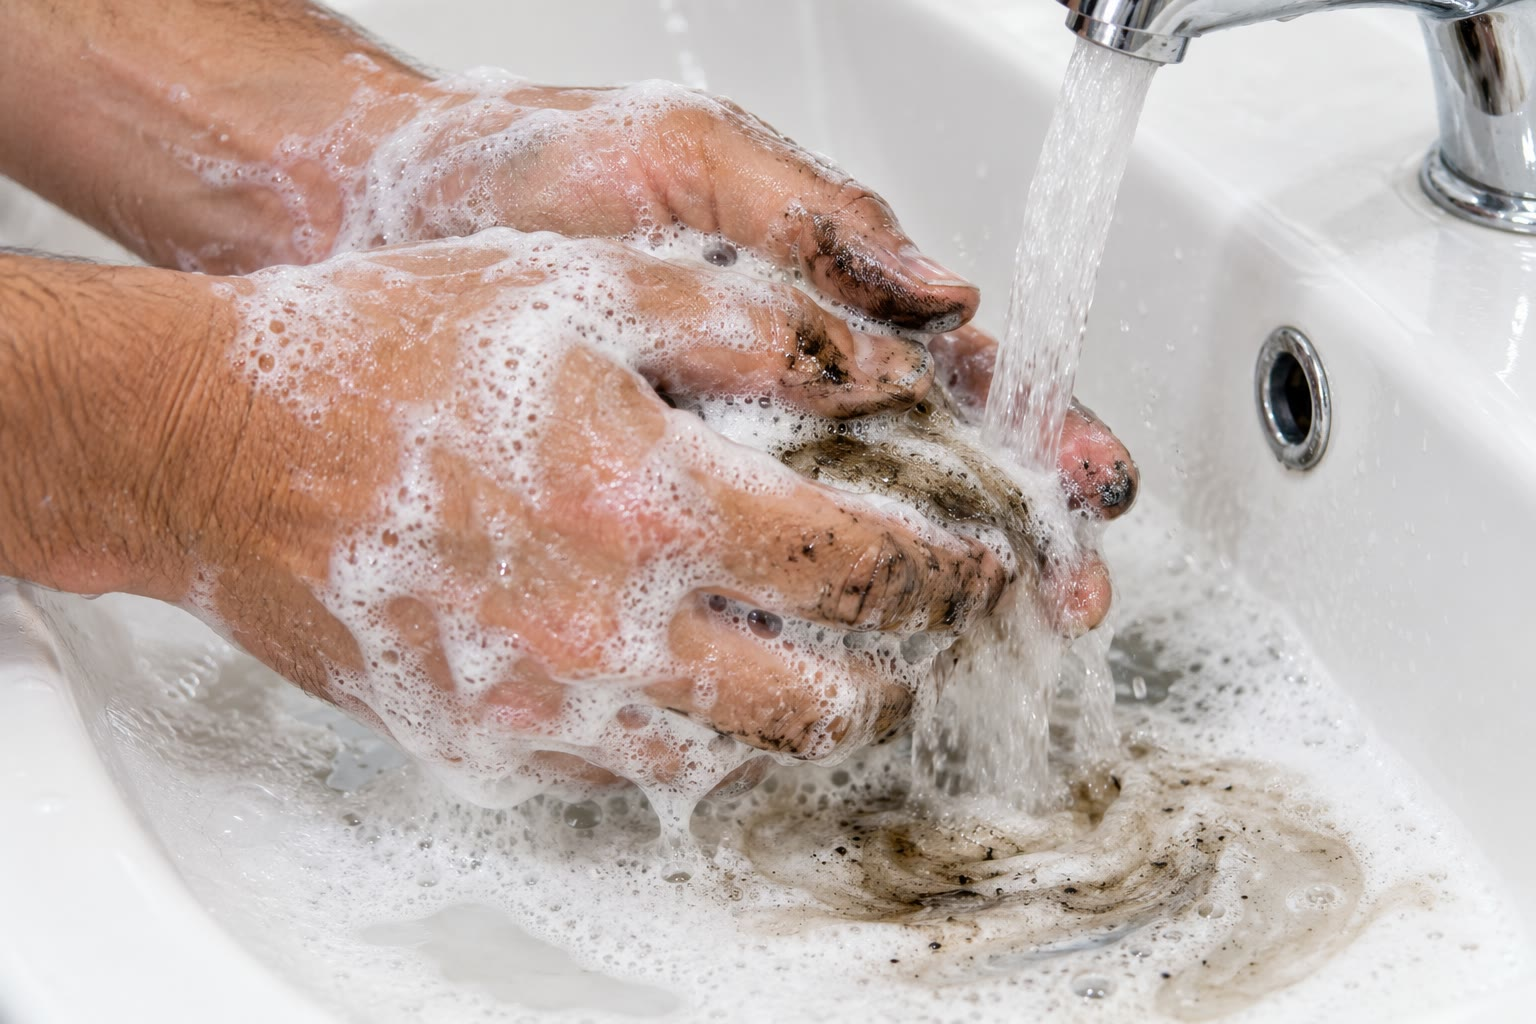
\includegraphics[width=0.48\linewidth]{images/book1/ai/g11-greasy-hands.jpg}

{\small Mencuci tangan yang berminyak: sabun membawa pergi lemaknya di
dalam \omterm{def:g11:dissolution:amphiphilic}{misel}.}
\end{omfigure}

\begin{remark}[Air sadah dan kerak sabun]\label{rem:g11:dissolution:scum}
Air sadah mengandung banyak \omterm{def:g9:ions:ion}{ion} kalsium \ce{Ca^{2+}} dan \omterm{def:g9:ions:ion}{ion} magnesium
\ce{Mg^{2+}}, yang terlarut dari batuan yang dilaluinya. Dengan \omterm{def:g9:ions:ion}{ion-ion}
stearat, \omterm{def:g9:ions:ion}{ion-ion} itu membentuk \omterm{def:g9:ions:precipitate}{endapan} (\cref{ch:g9:ions}), kalsium
stearat:
\[
  \ce{2C17H35COO- + Ca^{2+} -> Ca(C17H35COO)2(s)} .
\]
Padatan keabu-abuan ini adalah kerak sabun yang melingkari wastafel, dan
setiap \omterm{def:g9:ions:ion}{ion} sabun yang terperangkap di dalamnya hilang untuk mencuci: di
dalam air sadah, sabun sulit berbusa sampai cukup banyak sabun
ditambahkan untuk mengendapkan semua kalsiumnya.
\end{remark}

\begin{omfigure}
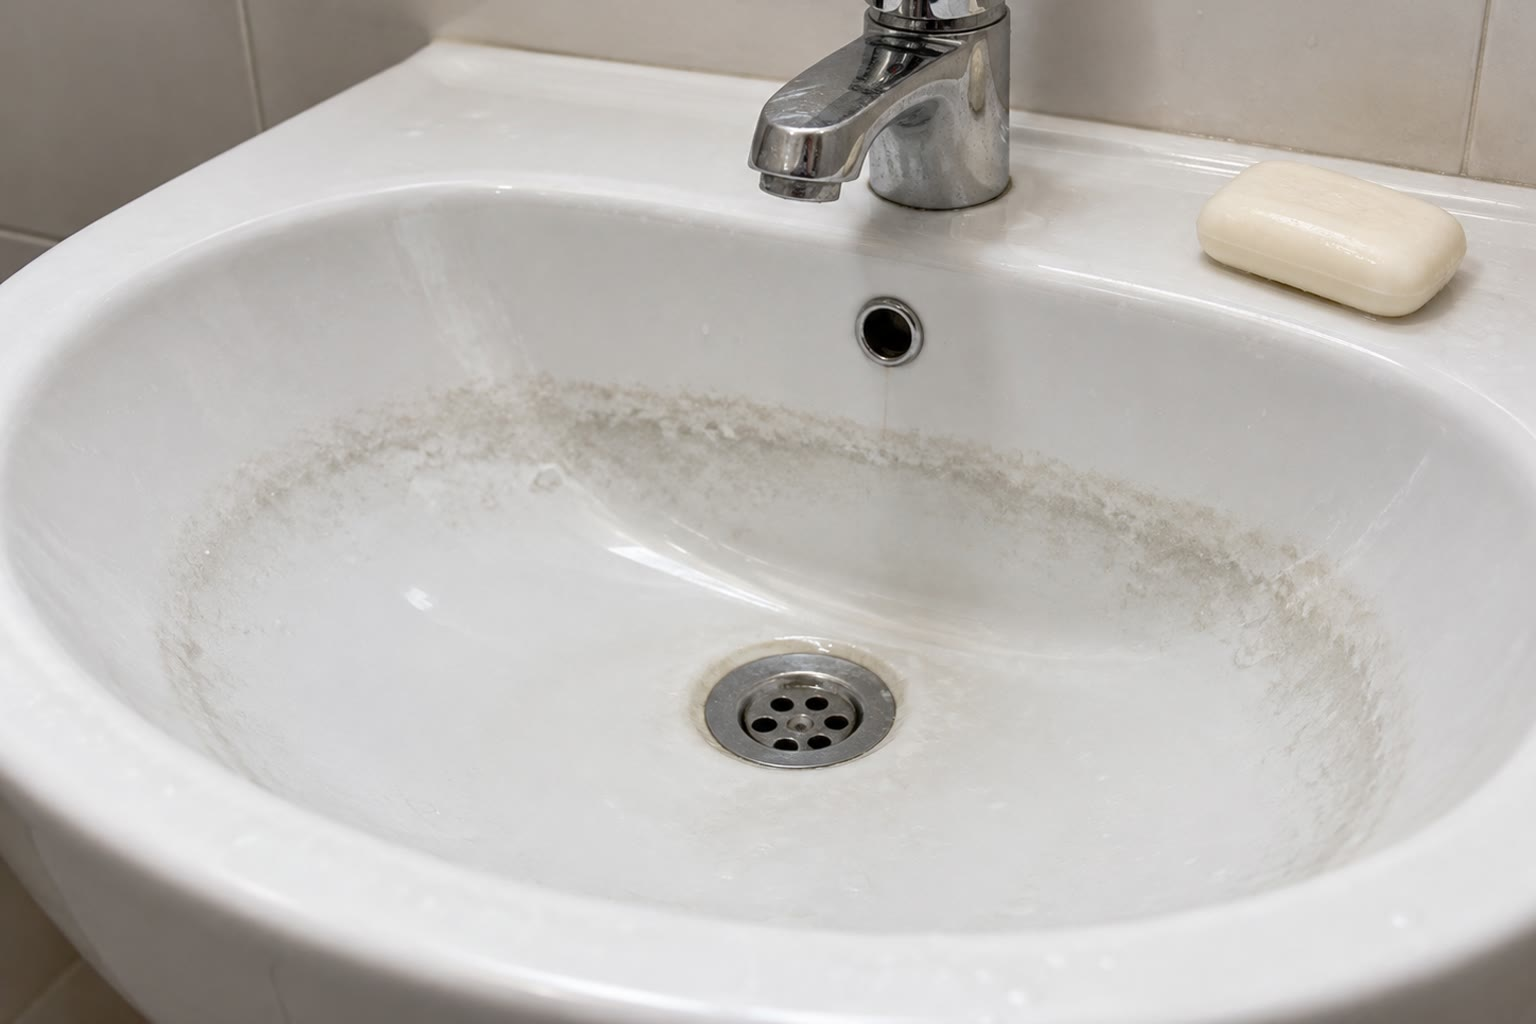
\includegraphics[width=0.45\linewidth]{images/book1/ai/g11-soap-scum.jpg}

{\small Kerak sabun di wastafel: kalsium stearat, yang diendapkan oleh
air sadah.}
\end{omfigure}

\section{Latihan}


\begin{exercise}[$\star$]\label{exo:g11:dissolution:1}
Tuliskan persamaan pelarutan dalam air untuk natrium klorida \ce{NaCl},
kalsium klorida \ce{CaCl2}, natrium sulfat \ce{Na2SO4}, dan aluminium
klorida \ce{AlCl3}.
\end{exercise}

\begin{exercise}[$\star$]\label{exo:g11:dissolution:2}
Larutan natrium sulfat memiliki $c = \qty{0.050}{mol/L}$. Berikan
konsentrasi \omterm{def:g9:ions:ion}{ion} natrium dan \omterm{def:g9:ions:ion}{ion} sulfatnya.
\end{exercise}

\begin{exercise}[$\star$]\label{exo:g11:dissolution:3}
Apa yang dimaksud dengan \omterm{def:g11:dissolution:solvation}{hidrasi} sebuah \omterm{def:g9:ions:ion}{ion}? Ujung mana dari \omterm{def:g7:atoms-and-molecules:molecule}{molekul} air
yang mengarah ke \omterm{def:g9:ions:ion}{kation}, dan mana yang ke \omterm{def:g9:ions:ion}{anion}? Mengapa?
\end{exercise}

\begin{exercise}[$\star$]\label{exo:g11:dissolution:4}
Sebanyak \qty{2.67}{g} aluminium klorida dilarutkan menjadi
\qty{200.0}{mL} larutan. Hitung konsentrasi larutan itu dan konsentrasi
setiap \omterm{def:g9:ions:ion}{ion}.
\end{exercise}

\begin{exercise}[$\star$]\label{exo:g11:dissolution:5}
Tandai setiap bagian \omterm{def:g9:ions:ion}{ion} stearat sebagai \omterm{def:g11:dissolution:hydrophilic}{hidrofilik} atau \omterm{def:g11:dissolution:hydrophilic}{hidrofobik}, dan
jelaskan mengapa.
\end{exercise}

\begin{exercise}[$\star\star$]\label{exo:g11:dissolution:6}
\omterm{def:g6:solutions-and-solubility:solute}{Pelarut} mana, air atau sikloheksana, yang akan kamu pilih untuk
melarutkan: garam; lilin (rantai hidrokarbon yang panjang); gula (banyak
gugus \ce{O-H}); iodin? Berikan alasan untuk setiap pilihan.
\end{exercise}

\begin{exercise}[$\star\star$]\label{exo:g11:dissolution:7}
Etanol \ce{CH3-CH2-OH} bercampur dengan air dalam segala perbandingan,
tetapi heksana \ce{C6H14} tidak bercampur dengan air. Jelaskan.
\end{exercise}

\begin{exercise}[$\star\star$]\label{exo:g11:dissolution:8}
Lihatlah gambar \omterm{def:g11:dissolution:amphiphilic}{misel}. Mengapa ekor-ekornya di dalam dan
kepala-kepalanya di luar? Mengapa dua \omterm{def:g11:dissolution:amphiphilic}{misel} tidak bergabung menjadi satu
tetes lemak yang lebih besar?
\end{exercise}

\begin{exercise}[$\star\star$]\label{exo:g11:dissolution:9}
Sebuah zat harum tumbuhan terlarut dalam air. Untuk mengekstraksinya,
seorang ahli kimia dapat memakai etanol atau sikloheksana. Mana yang
cocok, dan mengapa yang lain tidak (pikirkan kemampuan bercampurnya)?
\end{exercise}

\begin{exercise}[$\star\star$]\label{exo:g11:dissolution:10}
Pada \omterm{def:g10:chemical-species:extraction}{ekstraksi} iodin, mengapa lapisan sikloheksana berada di atas?
Lapisan mana yang dikeluarkan melalui keran? Di mana iodin berada pada
akhirnya?
\end{exercise}

\begin{exercise}[$\star\star$]\label{exo:g11:dissolution:11}
Larutan tembaga sulfat yang biru dikocok dengan sikloheksana. Apa yang
terjadi pada warna birunya? Jelaskan.
\end{exercise}

\begin{exercise}[$\star\star\star$]\label{exo:g11:dissolution:12}
Berapa massa kalsium klorida yang harus dilarutkan untuk membuat
\qty{250.0}{mL} larutan dengan $[\ce{Cl-}] = \qty{0.300}{mol/L}$?
\end{exercise}

\begin{exercise}[$\star\star\star$]\label{exo:g11:dissolution:13}
Sebuah sampel air laut ternyata mengandung \qty{0.010}{mol/L} \omterm{def:g9:ions:ion}{ion}
kalsium dan \qty{0.053}{mol/L} \omterm{def:g9:ions:ion}{ion} magnesium. Jelaskan mengapa sabun
biasa sangat sulit berbusa dalam air laut. Berapa banyak natrium
stearat yang akan diendapkan oleh \omterm{def:g9:ions:ion}{ion-ion} kalsium saja dalam satu liter
air laut?
\end{exercise}

\begin{exercise}[$\star\star\star$]\label{exo:g11:dissolution:14}
Sebanyak \qty{100.0}{mL} larutan natrium klorida \qty{0.20}{mol/L}
\omterm{def:g2:mixing-and-dissolving:mix}{dicampur} dengan \qty{100.0}{mL} larutan kalsium klorida
\qty{0.10}{mol/L}. Tidak terbentuk \omterm{def:g9:ions:precipitate}{endapan}. Hitung konsentrasi
\ce{Na+}, \ce{Ca^{2+}}, dan \ce{Cl-} dalam \omterm{def:g6:pure-substances-and-mixtures:mixture}{campuran} itu, lalu periksalah
bahwa \omterm{def:g6:pure-substances-and-mixtures:mixture}{campuran} itu netral.
\end{exercise}

\begin{exercise}[$\star\star\star$]\label{exo:g11:dissolution:15}
% ledger: sol:I2-water, sol:I2-heptane, rho:heptane
Iodin \omterm{def:g2:mixing-and-dissolving:dissolve}{larut} sekitar \qty{0.3}{g} per liter air dan \qty{17}{g} per
kilogram heptana. Massa jenis heptana sekitar \qty{0.68}{kg/L}. Berapa
kali lebih banyak iodin yang dapat ditampung satu liter heptana
dibandingkan satu liter air? Apa artinya bagi sebuah \omterm{def:g10:chemical-species:extraction}{ekstraksi}?
\end{exercise}

\section{Soal: Sabun dan Air Sadah}

\begin{problem}[{Soal akhir pekan --- berapa banyak sabun yang terbuang
menjadi kerak sabun dalam satu bak mandi air sadah?}]
\label{pb:g11:dissolution:1}
% ledger: aw:Ca, aw:Mg, aw:C, aw:H, aw:O, aw:Na
Sebuah air keran mengandung \qty{120}{mg} \omterm{def:g9:ions:ion}{ion} kalsium dan \qty{24}{mg}
\omterm{def:g9:ions:ion}{ion} magnesium per liter. Sebuah bak mandi diisi \qty{150}{L} air itu,
dan orang yang mandi memakai sabun yang terbuat dari natrium stearat,
\ce{C17H35COONa}.

\medskip
\noindent\textbf{Bagian I --- Isi air itu.}
\begin{enumerate}
  \item Dari mana \omterm{def:g9:ions:ion}{ion-ion} kalsium dan magnesium dalam air keran berasal?
  \item Hitung \omterm{def:g10:concentration-and-dilution:molar-concentration}{konsentrasi molar} \omterm{def:g9:ions:ion}{ion} kalsium dan \omterm{def:g9:ions:ion}{ion} magnesium.
  \item \omterm{def:g9:ions:ion}{Ion-ion} kalsium disertai \omterm{def:g9:ions:ion}{ion-ion} hidrogenkarbonat, \ce{HCO3-},
        seolah-olah kalsium hidrogenkarbonat \ce{Ca(HCO3)2} yang telah
        dilarutkan. Tuliskan persamaan pelarutan itu, lalu simpulkan
        konsentrasi \omterm{def:g9:ions:ion}{ion} hidrogenkarbonat yang menyertai kalsium.
  \item Berapa jumlah \omterm{def:g9:ions:ion}{ion} kalsium yang dikandung bak mandi itu?
\end{enumerate}

\medskip
\noindent\textbf{Bagian II --- Sabunnya.}
\begin{enumerate}[resume]
  \item Hitung \omterm{def:g10:the-mole:molar-mass}{massa molar} natrium stearat.
  \item Tuliskan persamaan pelarutannya dalam air.
  \item Bagian mana dari \omterm{def:g9:ions:ion}{ion} stearat yang \omterm{def:g11:dissolution:hydrophilic}{hidrofilik}, dan mana yang
        \omterm{def:g11:dissolution:hydrophilic}{hidrofobik}? Mengapa \omterm{def:g9:ions:ion}{ion} itu disebut \omterm{def:g11:dissolution:amphiphilic}{amfifilik}?
  \item Uraikan sebuah \omterm{def:g11:dissolution:amphiphilic}{misel}, lalu jelaskan bagaimana \omterm{def:g11:dissolution:amphiphilic}{misel}
        menghilangkan lemak dari kulit.
  \item Mengapa sabun harus dilarutkan dalam air, bukan dalam minyak,
        untuk mencuci?
\end{enumerate}

\medskip
\noindent\textbf{Bagian III --- Kerak sabun.}
\begin{enumerate}[resume]
  \item Tuliskan persamaan \omterm{def:g9:ions:precipitate}{reaksi pengendapan} kalsium stearat.
        Periksalah bahwa persamaan itu setara dalam muatan.
  \item Isilah \omterm{def:g10:reaction-progress-table:extent}{tabel kemajuan} untuk \qty{1.00}{L} air keran itu dan \omterm{def:g9:ions:ion}{ion}
        stearat yang berlebih. \omterm{def:g7:chemical-reactions:reactant}{Pereaksi} mana yang membatasi?
  \item Berapa jumlah \omterm{def:g9:ions:ion}{ion} stearat yang hilang per liter karena kalsium?
  \item Hitung \omterm{def:g10:the-mole:molar-mass}{massa molar} kalsium stearat, dan massa kerak sabun yang
        terbentuk per liter.
  \item Magnesium stearat mengendap dengan cara yang sama. Berapa jumlah
        stearat yang diambil \omterm{def:g9:ions:ion}{ion-ion} magnesium per liter?
\end{enumerate}

\medskip
\noindent\textbf{Bagian IV --- Bak mandi.}
\begin{enumerate}[resume]
  \item Berapa jumlah \omterm{def:g9:ions:ion}{ion} stearat yang diendapkan oleh kalsium dalam
        seluruh bak mandi?
  \item Berapa massa sabun itu?
  \item Jika magnesium ikut dihitung, berapa massa sabun yang terbuang
        seluruhnya?
  \item Sebatang sabun beratnya sekitar \qty{100}{g}. Berapa batang yang
        diambil oleh kalsium saja?
  \item Nyatakan jawaban akhirnya: berapa massa sabun yang dibuang oleh
        kalsium dalam satu bak mandi \qty{150}{L} air ini sebagai kerak
        sabun?
\end{enumerate}
\end{problem}
